%%%%%%%%%%%%%%%%%%%%%%%%%%%%%%%%%%%%%%%%%%%%%%%%%%%%%%%%%%%%%%%%%%%%%%%
% Ansys Techcon 2022 - API Guidance and Best Practices
%%%%%%%%%%%%%%%%%%%%%%%%%%%%%%%%%%%%%%%%%%%%%%%%%%%%%%%%%%%%%%%%%%%%%%%
\documentclass[t]{beamer}

\usetheme{Ansys2022}

\usepackage{bbding,pifont}
\usepackage{minted}
\usepackage{xcolor}
\usepackage{pdfpages}
\usepackage{listings}
\usepackage{hyperref}
\usepackage{etoolbox}
\AtBeginEnvironment{quote}{\par\singlespacing\small}

\usepackage{tikz}
\usetikzlibrary{intersections}
\usetikzlibrary{shapes.geometric, arrows,positioning}

\usepackage[edges]{forest}
\hypersetup{
    colorlinks=true,
    linkcolor=blue,
    filecolor=magenta,
    urlcolor=cyan,
}


\urlstyle{same}
\setbeamercolor{background canvas}{bg=}

\definecolor{bleudefrance}{rgb}{0.19, 0.55, 0.91}

%%%%%%%%%%%%%%%%%%%%%%%%%%%%%%%%%%%%%%%%%%%%%%%%%%%%%%%%%%%%%%%%%%%%%%%%%%%%%%%

\tikzset{
  startstop/.style={
    rectangle,
    rounded corners,
    minimum width=3cm,
    minimum height=0.75cm,
    align=center,
    draw=black,
    fill=ANSYS@Gold,
    },
  process/.style={
    rectangle,
    minimum width=3cm,
    minimum height=0.75cm,
    align=center,
    draw=black,
    fill=ANSYS@Blue,
    text=white,
    },
  decision/.style={
    diamond,
    aspect=4,
    minimum width=3cm,
    minimum height=1cm,
    align=center,
    draw=black,
    fill=ANSYS@Blue,
    text=white,
    },
  arrow/.style={thick,->,>=stealth},
  dec/.style={
    ellipse,
    align=center,
    draw=black,
    fill=ANSYS@Bronze,
    },
}

\begin{document}

%%%%%%%%%%%%%%%%%%%%%%%%%%%%%%%%%%%%%%%%%%%%%%%%%%%%%%%%%%%%%%%%%%%%%%%%%%%%%%%
%% Title Slide

\title{API Guidance and Best Practices}
%% \subtitle{}
\author{Alex Kaszynski \\ Roberto Pastor Muela}
\date{\today}

\titleframe{}


%%%%%%%%%%%%%%%%%%%%%%%%%%%%%%%%%%%%%%%%%%%%%%%%%%%%%%%%%%%%%%%%%%%%%%%%%%%%%%%
%% Table of contents

\begin{frame}{Table of Contents}
  \tableofcontents
  \vspace{200pt}  %% force top tight
\end{frame}


%%%%%%%%%%%%%%%%%%%%%%%%%%%%%%%%%%%%%%%%%%%%%%%%%%%%%%%%%%%%%%%%%%%%%%%%%%%%%%%
\section{Why APIs?}

\begin{frame}[fragile=singleslide]
  \frametitle{Remote API - Overview}
  \vspace{-10pt}

  \begin{itemize}
  \item Today, APIs are playing an increasingly important role in our lives.
  \item They provide the means for our computers to interact with the outside world, and they allow us to access information and services that we wouldn't otherwise be able to use.
  \item In the future, they will become even more important, as they will be used to control and manage our increasingly complex systems.
  \end{itemize}

  \begin{exampleblock}{API Example}
    This slide was entirely generated from an API based on this statement:


    \textit{``Public software APIs will be so fundamental to our modern
      products that will be unable to comprehend how we survived without
      them.''}

  \end{exampleblock}

\end{frame}

%%%%%%%%%%%%%%%%%%%%%%%%%%%%%%%%%%%%%%%%%%%%%%%%%%%%%%%%%%%%%%%%%%%%%%%%%%%%%%%
\subsection{OpenAI API Query}
\begin{frame}[fragile=singleslide]
  \frametitle{OpenAI API Query}

  \begin{itemize}
  \item POST a simple API query to OpenAI's GPT-3 API.
  \item Using the API defined at \href{https://beta.openai.com/docs/api-reference/completions/create?lang=curl}{OpenAI GPT-3 - API} to submit a \texttt{curl} request.
  \end{itemize}

  \begin{columns}[T]
    \begin{column}{.5\textwidth}
      \begin{exampleblock}{OpenAI API}
        \inputminted[fontsize=\footnotesize]{python}{code/openai_api.sh}
      \end{exampleblock}
    \end{column}

    \begin{column}{.5\textwidth}
      \centering
      \vspace{12pt}
      \href{https://asciinema.org/a/537661}{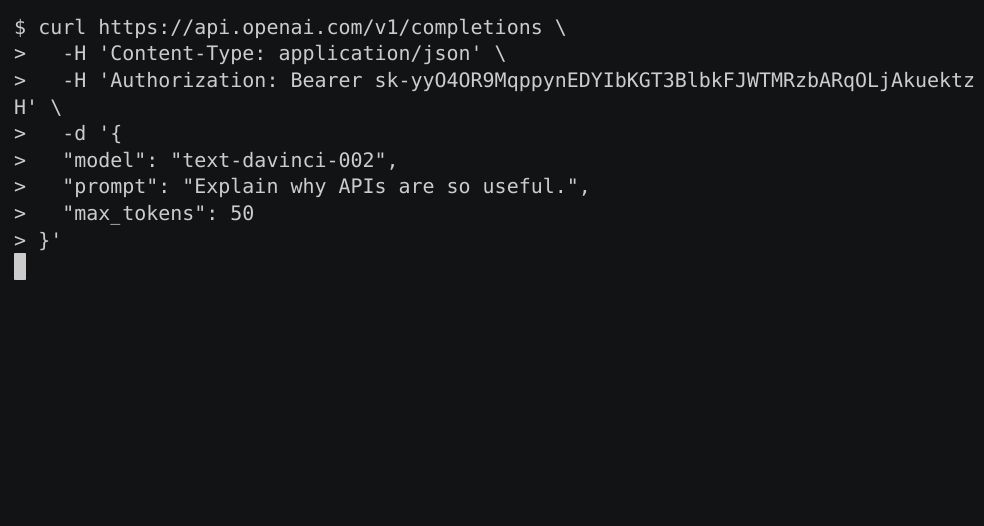
\includegraphics[width=0.9\textwidth]{figures/api-prompt.png}}
    \end{column}
  \end{columns}

\end{frame}

%%%%%%%%%%%%%%%%%%%%%%%%%%%%%%%%%%%%%%%%%%%%%%%%%%%%%%%%%%%%%%%%%%%%%%%%%%%%%%%
\begin{frame}[fragile=singleslide]
  \frametitle{OpenAI API Query - Python}

  Alternatively, you can use their Python client library to submit a request:

  \begin{exampleblock}{OpenAI API}
    \inputminted[fontsize=\footnotesize]{python}{code/openai_api.py}
  \end{exampleblock}
\end{frame}


%%%%%%%%%%%%%%%%%%%%%%%%%%%%%%%%%%%%%%%%%%%%%%%%%%%%%%%%%%%%%%%%%%%%%%%%%%%%%%%
\subsection{Problem Space}
\begin{frame}
  \frametitle{APIs - Problem Space}

  \begin{columns}[T]
    \begin{column}{.6\textwidth}

      %% The duration of this talk could easily be for a couple of hours, but
      %% since we only have 15 minutes, let's try to narrow the solution space to
      %% APIs and customer needs.

      \textbf{What do customers want?} Let's consider two kinds of customers
      who might want APIs:

      \begin{itemize}
      \item{Those who want to automate repetitive workflows.}
      \item{Those who need low-level access to the underlying libraries and
        components that make up an Ansys product.}
      \end{itemize}

      %% Companies used to spend a huge part of their resources in employees
      %% manually configuring and running simulations. Nowadays, most customers
      %% want to automate this process, such that by easily modifying an
      %% automated script they can rerun their simulations and evaluate the
      %% impact of these changes.

      %% Automation is a key point - having a person "behind the wheel" is
      %% sometimes necessary but once you have proven that your automation
      %% tools work, they are less error prone.

      \textbf{What do developers want?}

      \begin{itemize}
      \item{Well documented low-level interface to foreign libraries to avoid
        duplicating work.}
      \end{itemize}

      %% Developers use APIs all the time. These are the public interfaces that
      %% enable other developers to use their libraries.

    \end{column}

    \begin{column}{.45\textwidth}
      %% \centering
      \def\firstcircle{(0,0) circle (1.75cm)}
      \def\secondcircle{(60:2cm) circle (1.75cm)}
      \def\thirdcircle{(0:2cm) circle (1.75cm)}
      \begin{tikzpicture}
        \begin{scope}[shift={(3cm,-5cm)}, fill opacity=0.75]
          \fill[gray] \firstcircle;
          \fill[ANSYS@Bronze] \secondcircle;
          \fill[ANSYS@Blue] \thirdcircle;
          \draw \firstcircle node[below,text width=4cm,align=center,shift={(-2ex,0ex)}] {\footnotesize Product\\ Automation};
          \draw \secondcircle node [above,text width=4cm,align=center,shift={(0ex,2ex)}] {\footnotesize Low-Level\\ Access};
          \draw \thirdcircle node [below,text width=4cm,align=center,shift={(2ex,0ex)}] {\footnotesize Internal\\ Developers};
        \end{scope}
      \end{tikzpicture}
    \end{column}

  \end{columns}

\end{frame}


%%%%%%%%%%%%%%%%%%%%%%%%%%%%%%%%%%%%%%%%%%%%%%%%%%%%%%%%%%%%%%%%%%%%%%%%%%%%%%%
\begin{frame}
  \frametitle{APIs - Solution Space}

  \centering
  \def\firstcircle{(0,0) circle (2.0cm)}
  \def\secondcircle{(60:2.5cm) circle (2.0cm)}
  \def\thirdcircle{(0:2.5cm) circle (2.0cm)}
  \begin{tikzpicture}
    \begin{scope}[fill opacity=0.75]
      \fill[gray] \firstcircle;
      \fill[ANSYS@Bronze] \secondcircle;
      \fill[ANSYS@Blue] \thirdcircle;
      \draw \firstcircle node[below,text width=4cm,align=center,shift={(-3ex,0ex)}] {\small Product\\ Automation};
      \draw \secondcircle node [above,text width=4cm,align=center,shift={(0ex,3ex)}] {\small Low-Level\\ Access};
      \draw \thirdcircle node [below,text width=4cm,align=center,shift={(3ex,0ex)}] {\small Internal\\ Developers};

      \node[] at (1.235,0.8) {APIs};
      \node[] at (1.235,-0.5) {Plugins};
      \node[] at (2.3,1.3) {*.c,*.h};
      \node[] at (0.17,1.3) {Scripts};

    \end{scope}
  \end{tikzpicture}

\end{frame}


%%%%%%%%%%%%%%%%%%%%%%%%%%%%%%%%%%%%%%%%%%%%%%%%%%%%%%%%%%%%%%%%%%%%%%%%%%%%%%%
\transitionframe{APIs - Definition and Examples}
\section{APIs - Definition and Examples}

\begin{frame}
  \frametitle{APIs - Definition and Examples}
  \tableofcontents[currentsection]
  \vspace{200pt}  %% force top tight
\end{frame}

\subsection{Definition}
\begin{frame}
  \frametitle{API Definition}

  API stands for ``Application Programming Interface'' and is a set of
  functions and procedures allowing the creation of applications that access
  the features or data of an operating system, application, or other service.

  %% Idea of an API predates the term itself!
  %%
  %% In 1948 British computer developers of the early computer EDSAC. Stored
  %% subroutines for libraries on punched paper tape organized in a filing
  %% cabinet.
  %%
  %% This cabinet also contained what Wilkes and Wheeler called a
  %% "library catalog" of notes about each subroutine and how to incorporate it
  %% into a program.
  %%
  %% Today, such a catalog would be called an API (or an API
  %% specification or API documentation) because it instructs a programmer on
  %% how to call each subroutine.

  \begin{examples}
    \begin{itemize}
    \item A C header file
    \item Public Python class function
    \item RESTful HTTP API (POST, GET)
    \end{itemize}
  \end{examples}

  In essence, APIs let the users know how to interact with a given library or
  network interface without containing the specifics of the implementation.


\end{frame}


%%%%%%%%%%%%%%%%%%%%%%%%%%%%%%%%%%%%%%%%%%%%%%%%%%%%%%%%%%%%%%%%%%%%%%%%%%%%%%%
\subsection{Examples - Library Based}

\begin{frame}
  \frametitle{APIs in the Wild - C++ API}
  \vspace{-10pt}

  \href{https://vtk.org/doc/nightly/html/index.html}{VTK - API Reference}

  \centering
  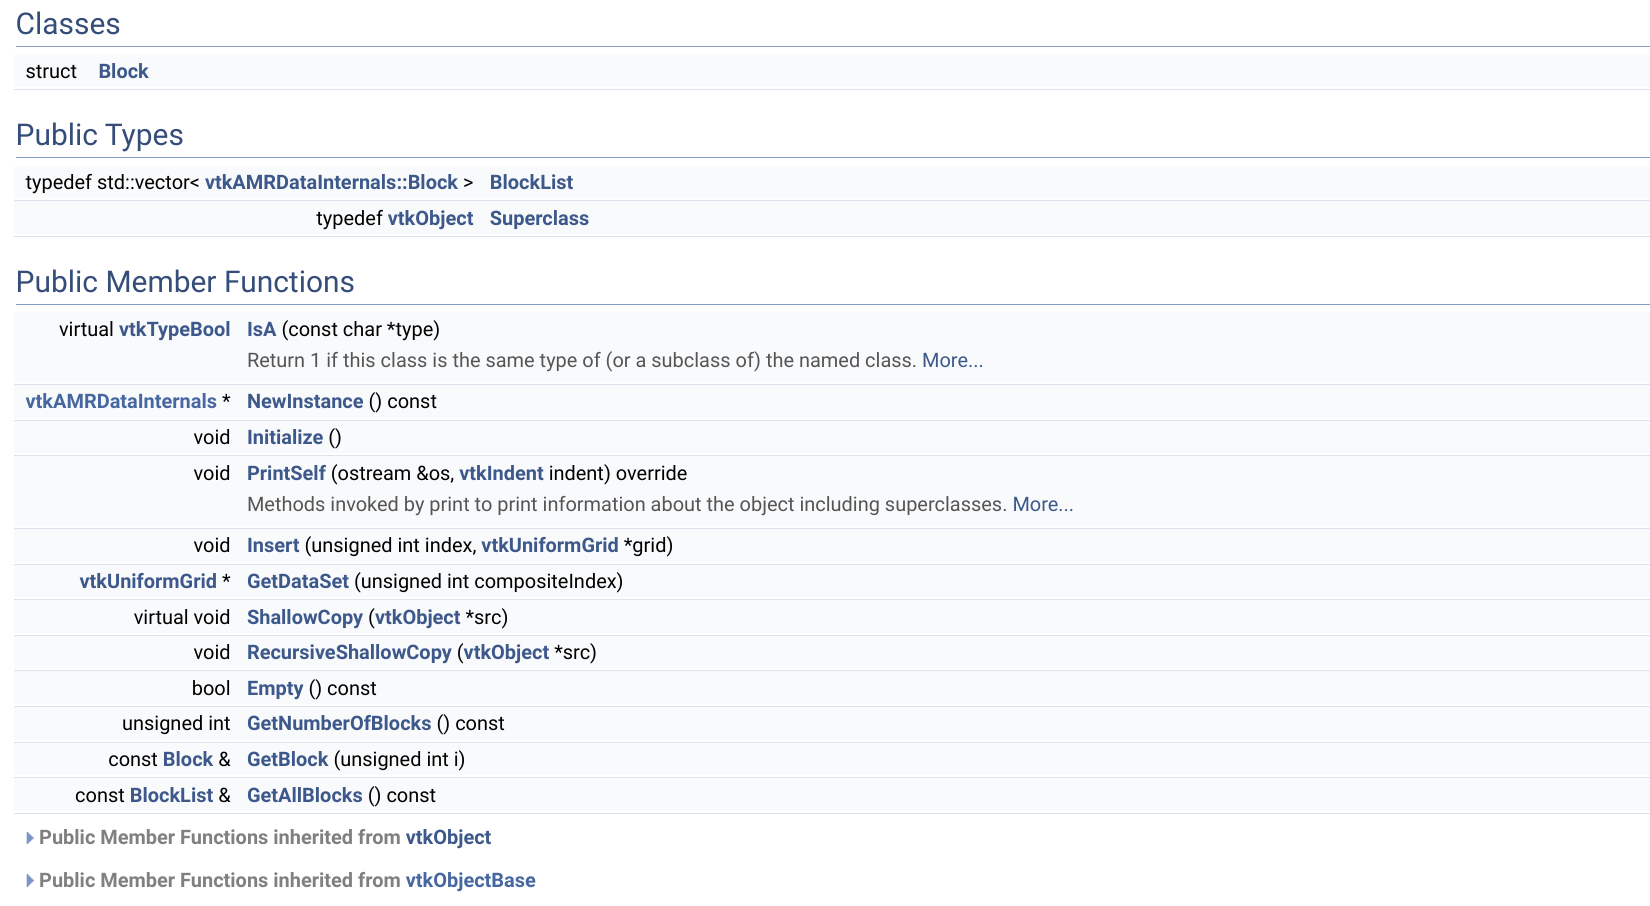
\includegraphics[height=.75\textheight]{./figures/vtk_api.png}

\end{frame}

%%%%%%%%%%%%%%%%%%%%%%%%%%%%%%%%%%%%%%%%%%%%%%%%%%%%%%%%%%%%%%%%%%%%%%%%%%%%%%%
\begin{frame}
  \frametitle{APIs in the Wild - Python API}
  \vspace{-10pt}

  \href{https://numpy.org/doc/stable/reference/}{NumPy - API Reference}

  \centering
  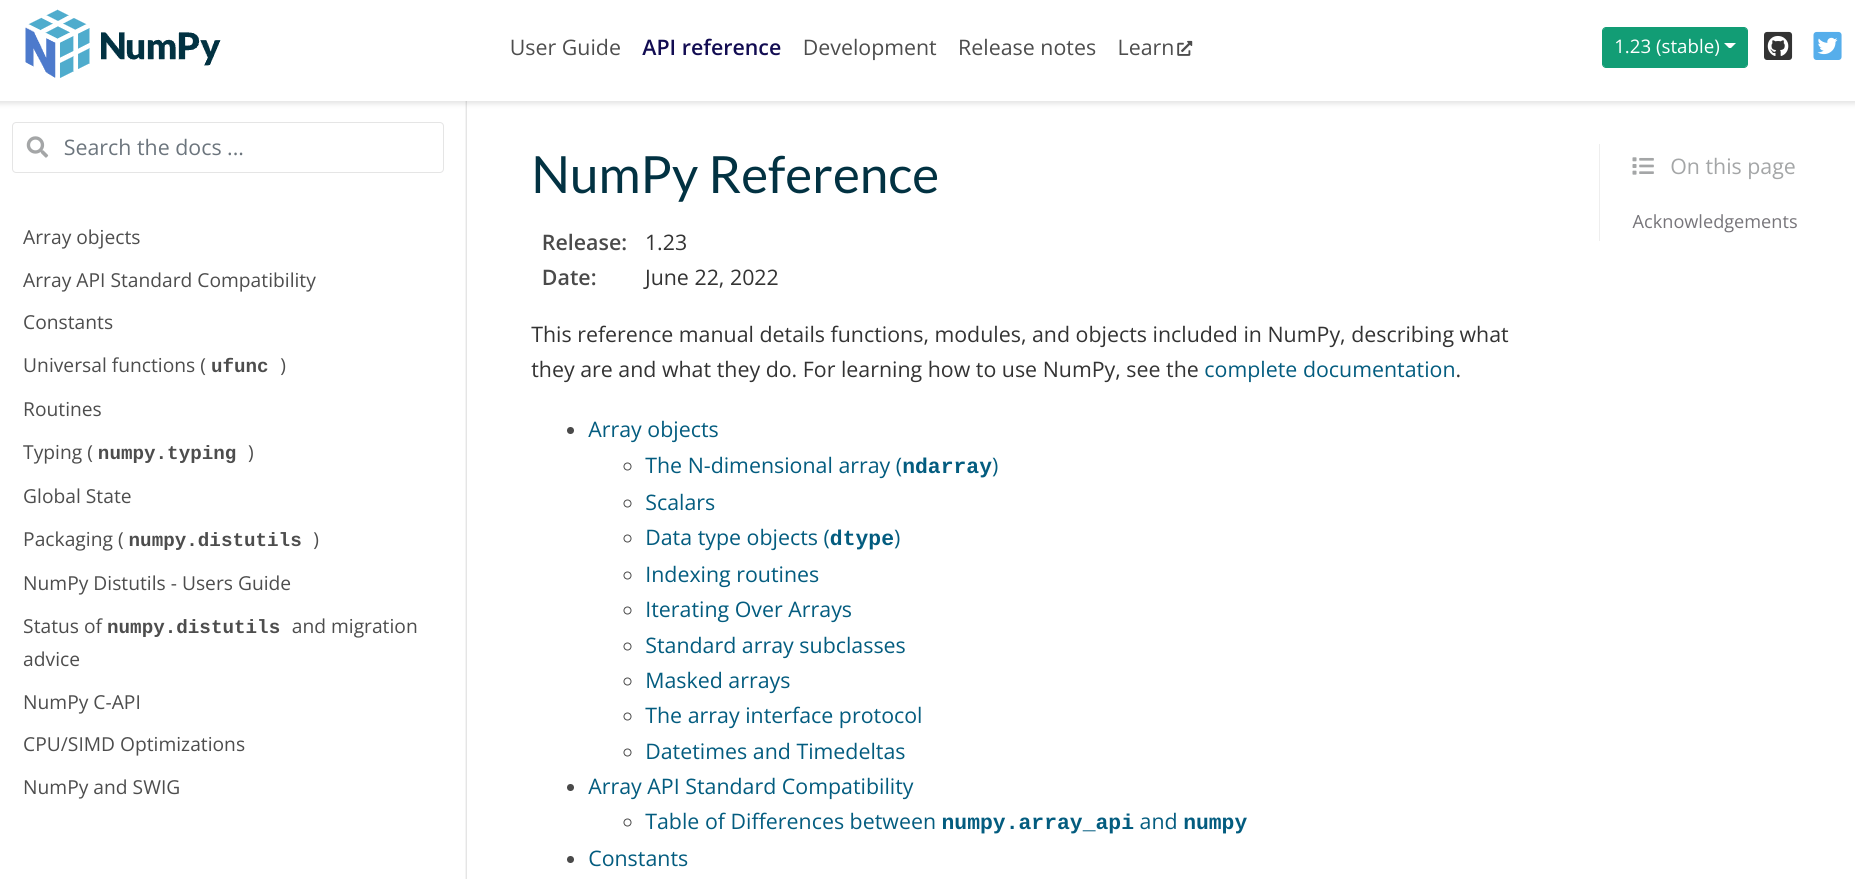
\includegraphics[height=.75\textheight]{./figures/numpy_api.png}

\end{frame}

\subsection{Examples - Network Based}


%%%%%%%%%%%%%%%%%%%%%%%%%%%%%%%%%%%%%%%%%%%%%%%%%%%%%%%%%%%%%%%%%%%%%%%%%%%%%%%
\begin{frame}
  \frametitle{APIs in the Wild - REST API}
  \vspace{-10pt}

  \href{https://beta.openai.com/docs/api-reference/completions/create?lang=python}{OpenAI - API Reference}

  \centering
  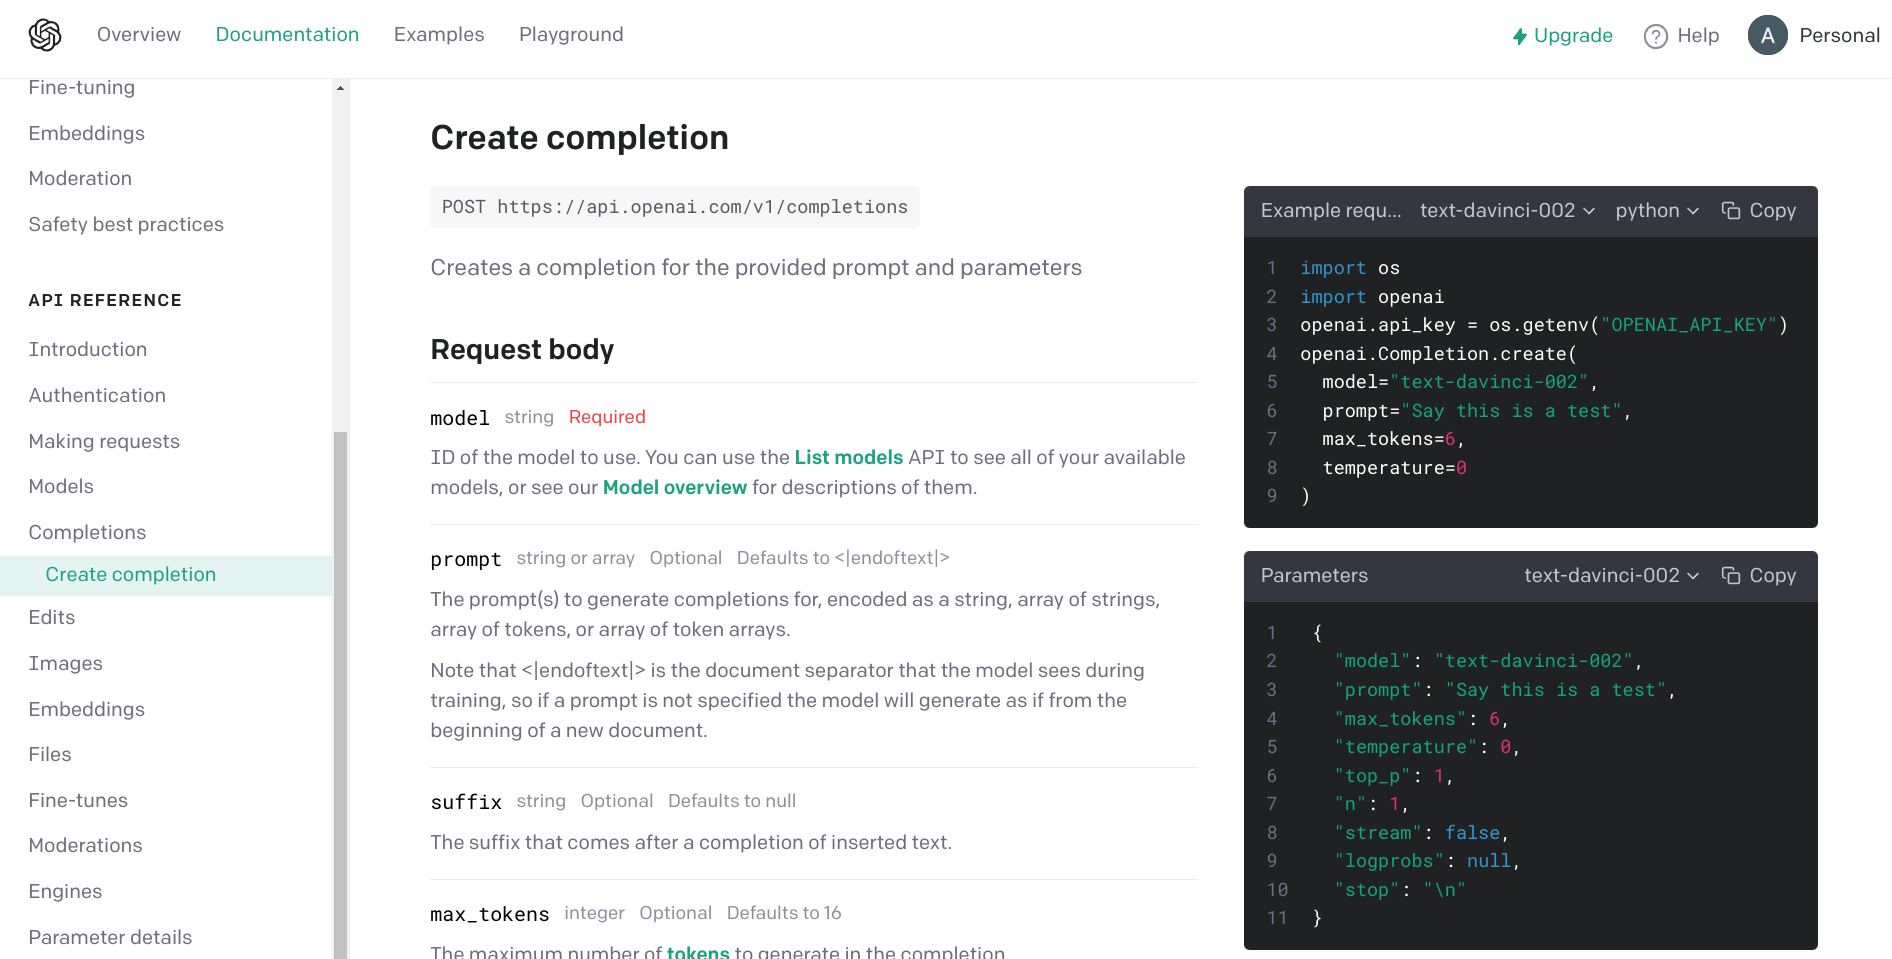
\includegraphics[height=.75\textheight]{./figures/openai-api.png}

\end{frame}

%%%%%%%%%%%%%%%%%%%%%%%%%%%%%%%%%%%%%%%%%%%%%%%%%%%%%%%%%%%%%%%%%%%%%%%%%%%%%%%
\transitionframe{Ansys's API - Local and Remote}
\section{Ansys's API - Local and Remote}

\begin{frame}
  \frametitle{APIs - Definition and Examples}
  \tableofcontents[currentsection]
  \vspace{200pt}  %% force top tight
\end{frame}

\begin{frame}
  \frametitle{Ansys's API - A Holistic Overview}

  To address the need for product automation and low-level access, we need to
  expose three types of APIs:

    \begin{itemize}
      \item Core service/library APIs
      \item Product automation APIs
      \item Remote product APIs
    \end{itemize}

    These three levels of APIs ensure Ansys can enable:

    \begin{itemize}
      \item Inter-product communication without writing to disk
      \item Product customization and automation
      \item Compatibility with cloud infrastructure (e.g. \href{https://www.docker.com/}{Docker})
    \end{itemize}

\end{frame}


%%%%%%%%%%%%%%%%%%%%%%%%%%%%%%%%%%%%%%%%%%%%%%%%%%%%%%%%%%%%%%%%%%%%%%%%%%%%%%%

\begin{frame}
  \frametitle{Ansys's Product APIs - Tech Stack}

  %% Simple pyramid
  \begin{tikzpicture}
    \coordinate (A) at (-4,0) {};
    \coordinate (B) at ( 4,0) {};
    \coordinate (C) at (0,6) {};
    \draw[name path=AC] (A) -- (C);
    \draw[name path=BC] (B) -- (C);
    \foreach \y/\A/\B\C in {
      0/Core Library API/Compiled/ 
\includegraphics[height=.1\textheight]{figures/c-logo.png} 
\includegraphics[height=.1\textheight]{figures/fortran-logo.png},
      2/Product Automation API/Interpreted/ 
\includegraphics[height=.1\textheight]{figures/python-logo.png},
      4/Remote API/Network/ 
\includegraphics[height=.1\textheight]{figures/rest-logo.png} 
\includegraphics[height=.1\textheight]{figures/grpc-logo.png}
    } {
      \path[name path=horiz] (A|-0,\y) -- (B|-0,\y);

      % Level of API
      \draw[name intersections={of=AC and horiz,by=P},
        name intersections={of=BC and horiz,by=Q}] (P) -- (Q)
      node[midway,above] {\A};

      % Language/Architecture
      \draw[name intersections={of=AC and horiz,by=P},
        name intersections={of=BC and horiz,by=Q}] (P) -- (Q)
      node[midway,above,shift={(28ex,0ex)}] {\B};

      % Image
      \draw[name intersections={of=AC and horiz,by=P},
        name intersections={of=BC and horiz,by=Q}] (P) -- (Q)
      node[midway,above,shift={(40ex,0ex)}] {\C};
    }
  \end{tikzpicture}

\end{frame}

%%%%%%%%%%%%%%%%%%%%%%%%%%%%%%%%%%%%%%%%%%%%%%%%%%%%%%%%%%%%%%%%%%%%%%%%%%%%%%%
% low-level part

\def\pyramidone{

  %% Stack pyramid
  \resizebox{.004\textwidth}{!}{
    \begin{tikzpicture}[overlay]
      \tikzset{shift={(current page.center)},xshift=39cm,yshift=-1cm}
    \coordinate (A) at (-4,0) {};
    \coordinate (B) at ( 4,0) {};
    \coordinate (C) at (0,6) {};
    \draw[name path=AC] (A) -- (C);
    \draw[name path=BC] (B) -- (C);
    \foreach \y/\A in {
      0/\color{ANSYS@Bronze} Core Library API,
      2/\color{lightgray} Product Automation API,
      4/\color{lightgray} Remote API/Network
    } {
      \path[name path=horiz] (A|-0,\y) -- (B|-0,\y);

      % Level of API
      \draw[name intersections={of=AC and horiz,by=P},
        name intersections={of=BC and horiz,by=Q}] (P) -- (Q);

      % Language/Architecture
      \draw[name intersections={of=AC and horiz,by=P},
        name intersections={of=BC and horiz,by=Q}] (P) -- (Q)
      node[midway,above,shift={(-40ex,0ex)}] {\huge \A};

    }
  \end{tikzpicture}
  }

}

%%%%%%%%%%%%%%%%%%%%%%%%%%%%%%%%%%%%%%%%%%%%%%%%%%%%%%%%%%%%%%%%%%%%%%%%%%%%%%%
\subsection{Core Library API}
\begin{frame}[fragile=singleslide]
  \frametitle{Core Library API - Overview}
  \vspace{-10pt}

  \begin{itemize}
  \item Primarily directed for developers and (rarely) customers wishing to customize at a very low-level.
  \item Core Library API should be exposed in the same language as the library source.
  \item Minimizes code overhead and duplication.
  \end{itemize}

  \vspace{2pt}
  \inputminted[fontsize=\tiny]{python}{code/fdresu.inc}

  \pyramidone

\end{frame}


%%%%%%%%%%%%%%%%%%%%%%%%%%%%%%%%%%%%%%%%%%%%%%%%%%%%%%%%%%%%%%%%%%%%%%%%%%%%%%%
% mid-level

\def\pyramidtwo{

  %% Stack pyramid
  \resizebox{.004\textwidth}{!}{
    \begin{tikzpicture}[overlay]
      \tikzset{shift={(current page.center)},xshift=39cm,yshift=-1.2cm}
    \coordinate (A) at (-4,0) {};
    \coordinate (B) at ( 4,0) {};
    \coordinate (C) at (0,6) {};
    \draw[name path=AC] (A) -- (C);
    \draw[name path=BC] (B) -- (C);
    \foreach \y/\A in {
      0/\color{lightgray} Core Library API,
      2/\color{ANSYS@Bronze} Product Automation API,
      4/\color{lightgray} Remote API/Network
    } {
      \path[name path=horiz] (A|-0,\y) -- (B|-0,\y);

      % Level of API
      \draw[name intersections={of=AC and horiz,by=P},
        name intersections={of=BC and horiz,by=Q}] (P) -- (Q);

      % Language/Architecture
      \draw[name intersections={of=AC and horiz,by=P},
        name intersections={of=BC and horiz,by=Q}] (P) -- (Q)
      node[midway,above,shift={(-40ex,0ex)}] {\huge \A};

    }
  \end{tikzpicture}
  }

}

%%%%%%%%%%%%%%%%%%%%%%%%%%%%%%%%%%%%%%%%%%%%%%%%%%%%%%%%%%%%%%%%%%%%%%%%%%%%%%%
\subsection{Product Customization and Automation}
\begin{frame}[fragile=singleslide]
  \frametitle{Product Customization and Automation - Overview}
  \vspace{-10pt}

  \begin{itemize}
  \item Directed at method developers who understand the product at the ``analyst'' level as well as understand basic programming.
  \item Target language should be a high-level interpreted language like Python or Julia.
  \item Python is one of the top languages used by method developers due to its
    wide and deep ecosystem of libraries, frameworks, and tools.
  \end{itemize}

  \href{https://www.tiobe.com/tiobe-index/}{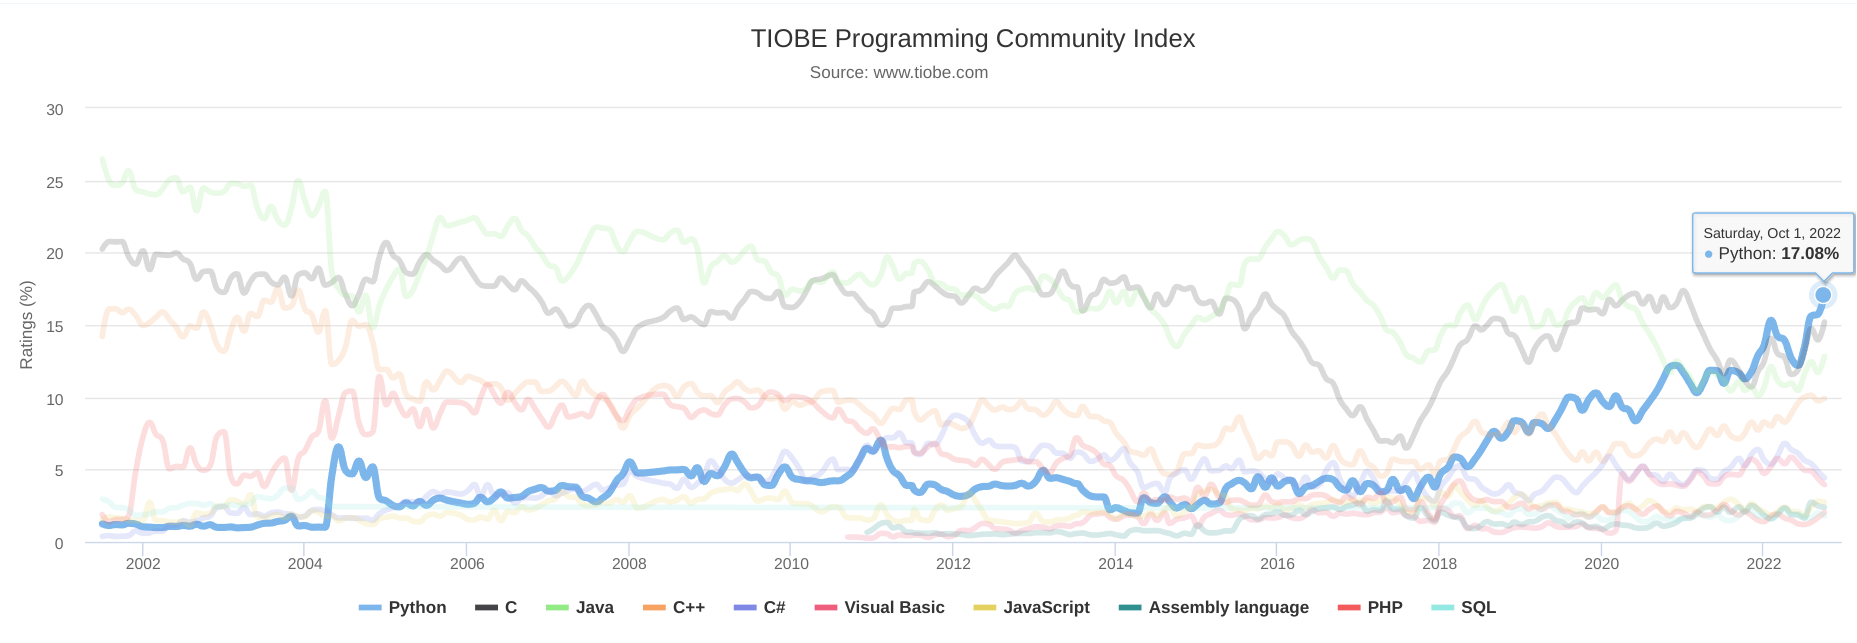
\includegraphics[height=.4\textheight]{./figures/tiobe_index.png}}

  \pyramidtwo

\end{frame}


%%%%%%%%%%%%%%%%%%%%%%%%%%%%%%%%%%%%%%%%%%%%%%%%%%%%%%%%%%%%%%%%%%%%%%%%%%%%%%%

\begin{frame}[fragile=singleslide]
  \frametitle{Product Customization and Automation - Example}
  \vspace{-10pt}

  \begin{columns}[T]
    \begin{column}{.5\textwidth}
      \vspace{-5pt}
      \inputminted[fontsize=\footnotesize]{python}{code/pymapdl_example.py}
    \end{column}

    \begin{column}{.5\textwidth}
      \centering
      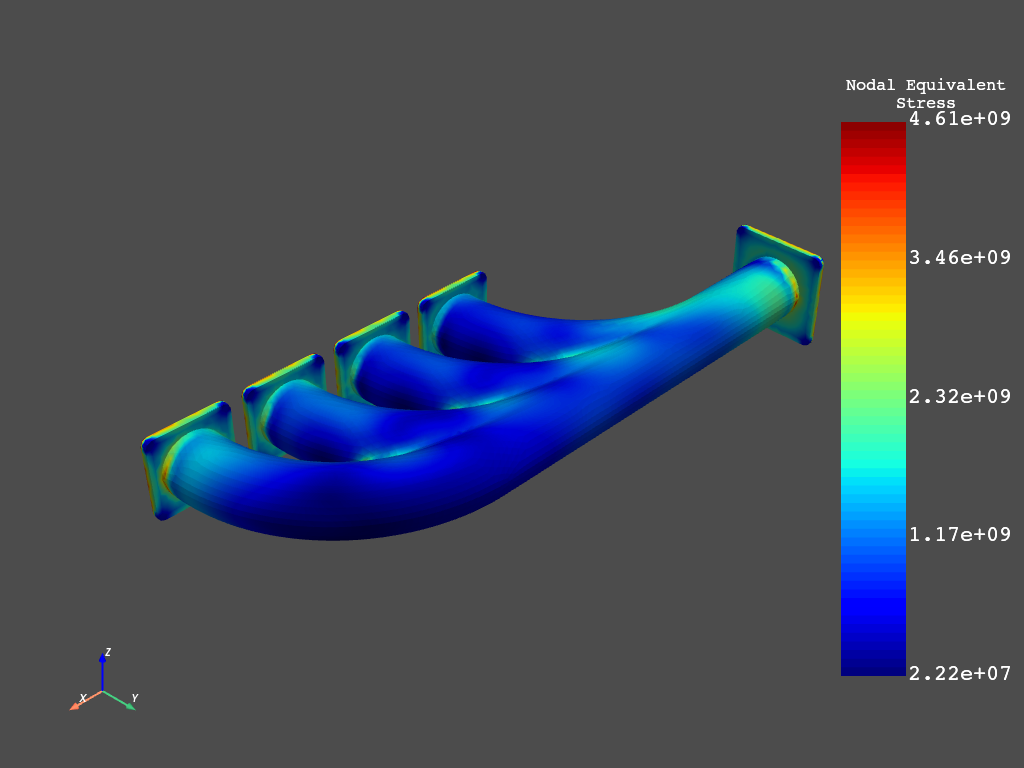
\includegraphics[height=5cm]{figures/sphx_glr_exhaust_manifold_thermal_stress_002.png}
    \end{column}

  \end{columns}

\end{frame}


%%%%%%%%%%%%%%%%%%%%%%%%%%%%%%%%%%%%%%%%%%%%%%%%%%%%%%%%%%%%%%%%%%%%%%%%%%%%%%%
% top-level

\def\pyramidthree{

  %% Stack pyramid
  \resizebox{.004\textwidth}{!}{
    \begin{tikzpicture}[overlay]
      \tikzset{shift={(current page.center)},xshift=39cm,yshift=-11.5cm}
    \coordinate (A) at (-4,0) {};
    \coordinate (B) at ( 4,0) {};
    \coordinate (C) at (0,6) {};
    \draw[name path=AC] (A) -- (C);
    \draw[name path=BC] (B) -- (C);
    \foreach \y/\A in {
      0/\color{lightgray} Core Library API,
      2/\color{lightgray} Product Automation API,
      4/\color{ANSYS@Bronze} Remote API/Network
    } {
      \path[name path=horiz] (A|-0,\y) -- (B|-0,\y);

      % Level of API
      \draw[name intersections={of=AC and horiz,by=P},
        name intersections={of=BC and horiz,by=Q}] (P) -- (Q);

      % Language/Architecture
      \draw[name intersections={of=AC and horiz,by=P},
        name intersections={of=BC and horiz,by=Q}] (P) -- (Q)
      node[midway,above,shift={(-40ex,0ex)}] {\huge \A};

    }
  \end{tikzpicture}
  }

}

%%%%%%%%%%%%%%%%%%%%%%%%%%%%%%%%%%%%%%%%%%%%%%%%%%%%%%%%%%%%%%%%%%%%%%%%%%%%%%%
\subsection{Remote API}
\begin{frame}[fragile=singleslide]
  \frametitle{Remote API - Overview}
  \vspace{-10pt}

  \begin{itemize}
  \item Consider two types of Remote APIs:
    \begin{itemize}
    \item{Inter-product communication: Use an architecture designed to allow
      the manipulation and exchange of information between multiple
      technologies and componentized software
      components. The \href{https://grpc.io/}{gRPC framework} works well for this
      scenario.}
    \item{Web APIs: Use an architecture designed for the interaction of
       physically separate components. \href{https://restfulapi.net/}{REST} is
       an ideal architectural style given its stateless, cacheable nature.}
    \end{itemize}
  \item The choice of the underlying architecture and technology must be driven
    by the problem and there is no ``one size fits all'' solution.
  \end{itemize}

  \pyramidthree{}

  %% Get example on the left
  \vspace{-20pt}
  \begin{columns}[T]
    \begin{column}{.6\textwidth}
      \begin{exampleblock}{\small Example REST Call}
        \begin{lstlisting}[basicstyle=\scriptsize]
curl -X POST "http://127.0.0.1:5000/Vectors" \
  -H "Content-Type: application/json" \
  -d '{"value":[5, 23, 3, 4]}'
        \end{lstlisting}
      \end{exampleblock}
    \end{column}
    \begin{column}{.2\textwidth}
    \end{column}
  \end{columns}

\end{frame}


%%%%%%%%%%%%%%%%%%%%%%%%%%%%%%%%%%%%%%%%%%%%%%%%%%%%%%%%%%%%%%%%%%%%%%%%%%%%%%%
\subsection{Remote API}
\begin{frame}[fragile=singleslide]
  \frametitle{Remote API - Lessons Learned}
  \vspace{-10pt}

  \begin{itemize}
  \item Web-facing APIs must reply on an abstraction layer that exposes only what is necessary to accomplish the task.
    \begin{itemize}
    \item An extended audience for your APIs.
    \item APIs can be reused to support new digital products.
    \item Normalized, consistent and well-governed API code and documentation.
    \item Flexibility on alternative/future coding standards and formats.
    \end{itemize}
  \item This will require the same sort of refactoring and abstracting as when
    exposing Ansys's products as GUIs. However, this time we need to consider
    both human and computers as ``first class'' users.
  \end{itemize}

  \vspace{-15pt}
  \pyramidthree{}

  %% Get example on the left
  \vspace{-5pt}
  \begin{columns}[T]
    \begin{column}{.6\textwidth}
      \begin{exampleblock}{\small Abstracted API}
        \inputminted[fontsize=\scriptsize]{python}{code/sample_apis.py}
      \end{exampleblock}
    \end{column}
    \begin{column}{.2\textwidth}
    \end{column}
  \end{columns}

\end{frame}


%%%%%%%%%%%%%%%%%%%%%%%%%%%%%%%%%%%%%%%%%%%%%%%%%%%%%%%%%%%%%%%%%%%%%%%%%%%%%%%
\begin{frame}[fragile=singleslide]
  \frametitle{Remote API - Example}
  \vspace{-10pt}

  \begin{columns}[T]
    \begin{column}{.6\textwidth}
      \vspace{-5pt}
      \begin{itemize}
      \item{We have an example for you at
        \href{https://apieigen.docs.ansys.com/index.html}{API Eigen Example}}
      \item{Includes:}
        \begin{itemize}
        \item{C++ REST Server and Client}
        \item{C++ gRPC Server and Client}
        \item{Python REST Server and Client}
        \item{Python gRPC Server and Client}
        \end{itemize}
      \item{Example designed to expose you to the basics of library-orientated
        remote APIs}
      \end{itemize}
    \end{column}

    \begin{column}{.45\textwidth}
      \centering
      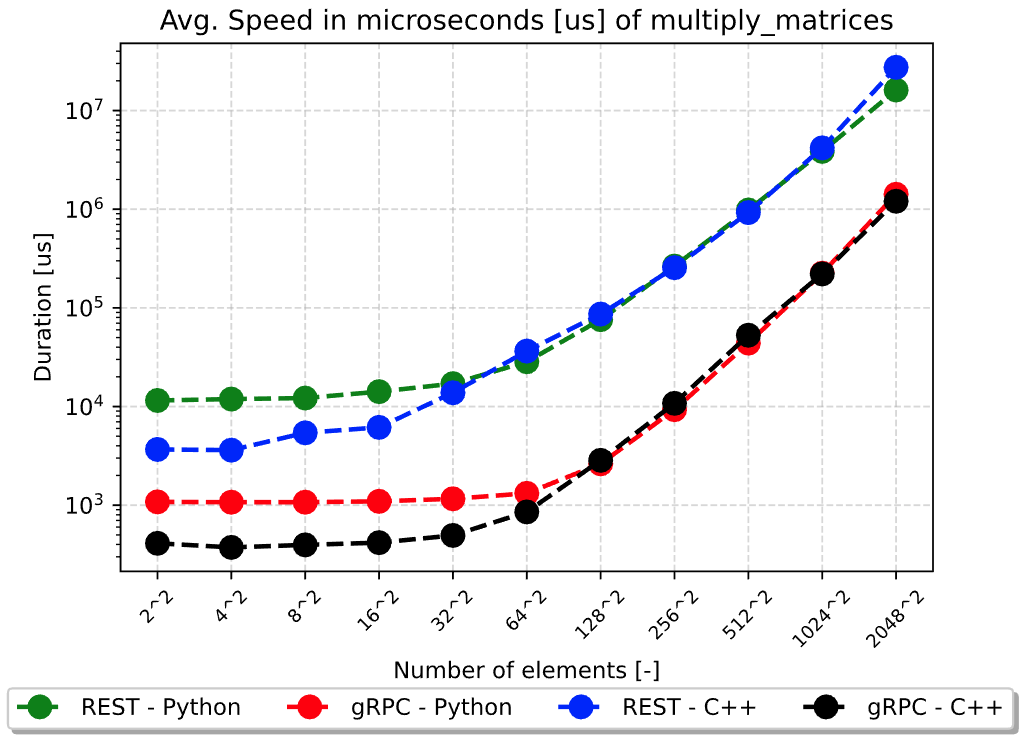
\includegraphics[height=4.5cm]{figures/api-benchmark.png}
    \end{column}

  \end{columns}

      \begin{example}
      \vspace{-5pt}
        \begin{lstlisting}[basicstyle=\tiny]
>>> import ansys.eigen.python.rest.server as rest_server
>>> app = rest_server.create_app()
>>> app.run("127.0.0.1", 5000)
        \end{lstlisting}
        \vspace{-5pt}
      \end{example}

\end{frame}

%%%%%%%%%%%%%%%%%%%%%%%%%%%%%%%%%%%%%%%%%%%%%%%%%%%%%%%%%%%%%%%%%%%%%%%%%%%%%%%
\lastframe{}

\end{document}
